\section{Задание:}
\textbf{Задание 1:} Сверстать страницу, максимально похожую на выбранную страницу из журнала «Квант»\\
\textbf{Задание 2:}\\
1. Рассчитать номер варианта по следующей схеме:\\
Ф – количество букв в фамилии, И – количество букв в имени\\
\text{Номер варианта} = 1 + (Ф $\times$ И) $\mod$ 8\\
2. Выполнить задание из полученного варианта, используя средства \LaTeX\\
Вариант 1\\
Работа с пакетом TikZ\\
\texttt{$\backslash$usepackage{tikz}}\\
\texttt{$\backslash$usetikzlibrary{automata,positioning}}\\
Воспроизвести диаграмму состояний (граф переходов) конечного автомата (англ.\\
Finite-state machine). Допускаются различия в расположении подписей над\\
переходами и во внешнем виде стрелок.\\
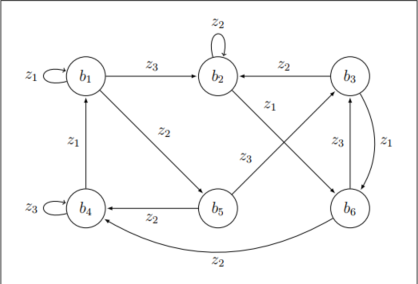
\includegraphics[width=\linewidth]{task2.png}\\
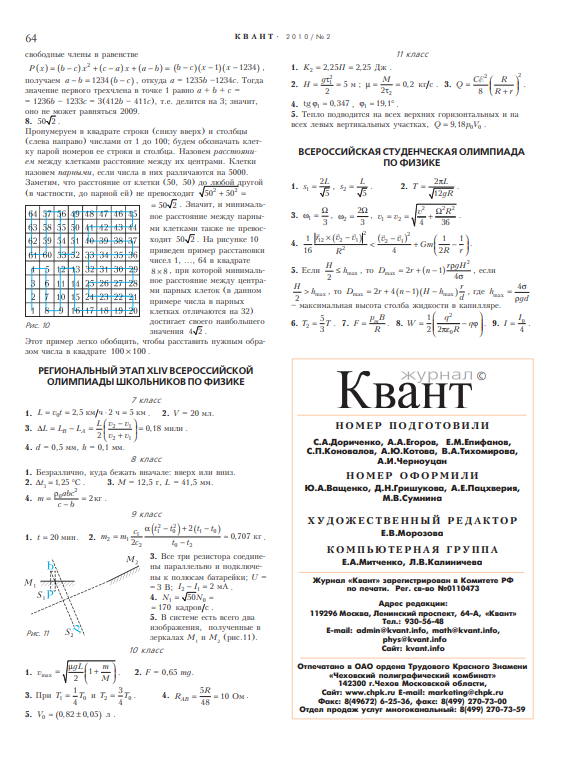
\includegraphics[width=\linewidth]{task 1.png}\\
\section{Отчет:}
\href{https://github.com/PNT1319star/Informatics}{Link to my GitHub}
\section{Результат:}
\newpage